\documentclass[12pt]{article}

\usepackage{sbc-template}

\usepackage{graphicx,url}

% !TeX encoding = UTF-8
\usepackage[utf8]{inputenc}
     
\sloppy

\title{Engenharia de Software em Cenário Crítico: Relato de Experiência na Implementação
da Arquitetura Offline-First no Aplicativo Móvel UFLA-IMA para Emergências Sanitárias.}

\author{
  Gustavo S. Silva\inst{1}, 
  Ahmed A. A. Esmin\inst{1}, 
  Marluce R. Pereira\inst{1}, 
  Igor E. de Carvalho\inst{1}
}


\address{
  Departamento de Ciência da Computação -- Universidade Federal de Lavras
  (UFLA)\\
  Caixa Postal 15.064 -- 37.200-000 -- Lavras -- MG -- Brazil
}

\begin{document} 

\maketitle

\begin{abstract}
  This meta-paper describes the style to be used in articles and short papers
  for SBC conferences. For papers in English, you should add just an abstract
  while for the papers in Portuguese, we also ask for an abstract in
  Portuguese (``resumo''). In both cases, abstracts should not have more than
  10 lines and must be in the first page of the paper.
\end{abstract}
     
\begin{resumo} 
  Este meta-artigo descreve o estilo a ser usado na confecção de artigos e
  resumos de artigos para publicação nos anais das conferências organizadas
  pela SBC. É solicitada a escrita de resumo e abstract apenas para os artigos
  escritos em português. Artigos em inglês deverão apresentar apenas abstract.
  Nos dois casos, o autor deve tomar cuidado para que o resumo (e o abstract)
  não ultrapassem 10 linhas cada, sendo que ambos devem estar na primeira
  página do artigo.
\end{resumo}


\section{Introdução}

A aplicação de boas práticas de Engenharia de Software é fundamental para assegurar a qualidade, 
manutenibilidade e sustentabilidade de sistemas computacionais. Em contextos governamentais, como 
o da vigilância sanitária agropecuária, onde a confiabilidade e a longevidade dos sistemas são 
requisitos críticos, tais práticas tornam-se ainda mais relevantes. O desafio se intensifica no 
desenvolvimento de Sistemas de Informação Móveis (SIMs), que devem garantir a coleta de dados em 
campo de forma eficaz, muitas vezes em ambientes com conectividade de rede limitada ou inexistente.

Este trabalho, portanto, apresenta um relato de experiência sobre o desenvolvimento e implementação do aplicativo móvel de Suporte a Emergências Sanitárias, fruto da parceria entre a Universidade Federal de Lavras (UFLA) e o Instituto Mineiro de Agropecuária (IMA). Com foco na aplicação de princípios de engenharia em um cenário de alta restrição, o projeto foi marcado por um prazo crítico de desenvolvimento (três meses) e pela exigência técnica fundamental de uma arquitetura Offline-First.

O relato detalha como a metodologia ágil (Scrum) foi adotada para gerenciar o projeto e permitir entregas funcionais sob pressão. Descreve-se a validação do aplicativo em um Simulado de Emergência Sanitária, que serviu como prova de conceito e permitiu a correção rápida de funcionalidades.

Na sequência, detalham-se as diretrizes de engenharia aplicadas ao desenvolvimento móvel. Aborda-se a escolha da Clean Architecture (Arquitetura Limpa) como estratégia para gerenciar a complexidade, desacoplar componentes e facilitar a manutenção. O núcleo técnico do relato foca nos desafios de implementação do fluxo Offline-First, incluindo a estratégia de persistência local, a integração com um backend existente e o mecanismo de sincronização de dados.

Por fim, o trabalho analisa os aprendizados obtidos, com foco principal no balanço entre a arquitetura de software ideal e o pragmatismo exigido pela restrição de tempo. Sistematizam-se as boas práticas de colaboração e gestão de versão (Git) e discute-se como a Tríplice Restrição (Escopo, Tempo e Custo) foi gerenciada para preservar a qualidade da entrega.

O restante deste Relato de Experiência está organizado como a seguir. A Seção 2 (Referencial Teórico) apresenta os conceitos fundamentais que embasam o projeto, como Metodologias Ágeis (Scrum) e os princípios da Clean Architecture. A Seção 3 (Contexto da Experiência e Metodologia) descreve o ambiente do projeto, a parceria UFLA-IMA e a aplicação prática do Scrum. A Seção 4 (Arquitetura Mobile e Desafios Técnicos) apresenta e justifica as decisões de engenharia, com foco na arquitetura Offline-First e na adaptação ao backend. A Seção 5 (Análise, Resultados e Aprendizados) discute os trade-offs entre pragmatismo e qualidade de código. Por fim, a Seção 6 (Considerações Finais) sistematiza as conclusões, contribuições e aprendizados do trabalho.

\section{Referencial Teórico} \label{sec:firstpage}

The first page must display the paper title, the name and address of the
authors, the abstract in English and ``resumo'' in Portuguese (``resumos'' are
required only for papers written in Portuguese). The title must be centered
over the whole page, in 16 point boldface font and with 12 points of space
before itself. Author names must be centered in 12 point font, bold, all of
them disposed in the same line, separated by commas and with 12 points of
space after the title. Addresses must be centered in 12 point font, also with
12 points of space after the authors' names. E-mail addresses should be
written using font Courier New, 10 point nominal size, with 6 points of space
before and 6 points of space after.

The abstract and ``resumo'' (if is the case) must be in 12 point Times font,
indented 0.8cm on both sides. The word \textbf{Abstract} and \textbf{Resumo},
should be written in boldface and must precede the text.

\section{Contexto da Experiência e Metodologia}

In some conferences, the papers are published on CD-ROM while only the
abstract is published in the printed Proceedings. In this case, authors are
invited to prepare two final versions of the paper. One, complete, to be
published on the CD and the other, containing only the first page, with
abstract and ``resumo'' (for papers in Portuguese).

\section{Arquitetura Mobile e Desafios Técnicos}

Section titles must be in boldface, 13pt, flush left. There should be an extra
12 pt of space before each title. Section numbering is optional. The first
paragraph of each section should not be indented, while the first lines of
subsequent paragraphs should be indented by 1.27 cm.

\subsection{Clean Architecture}

The subsection titles must be in boldface, 12pt, flush left.

\subsection{Offline-First}

Placeholder for Offline-First content.

\subsection{Desafios}

Placeholder for Desafios content.

\section{Análise, Resultados e Aprendizados}

Placeholder for Análise, Resultados e Aprendizados content.

\section{Figures and Captions}\label{sec:figs}


Figure and table captions should be centered if less than one line
(Figure~\ref{fig:exampleFig1}), otherwise justified and indented by 0.8cm on
both margins, as shown in Figure~\ref{fig:exampleFig2}. The caption font must
be Helvetica, 10 point, boldface, with 6 points of space before and after each
caption.

\begin{figure}[ht]
\centering
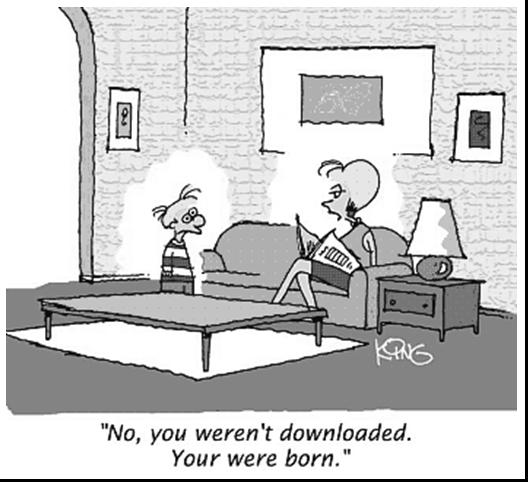
\includegraphics[width=.5\textwidth]{fig1.jpg}
\caption{A typical figure}
\label{fig:exampleFig1}
\end{figure}

\begin{figure}[ht]
\centering
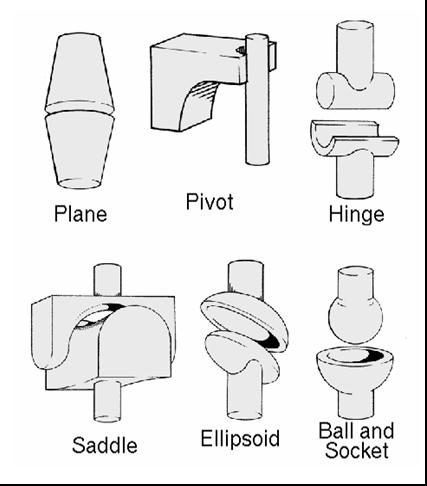
\includegraphics[width=.3\textwidth]{fig2.jpg}
\caption{This figure is an example of a figure caption taking more than one
  line and justified considering margins mentioned in Section~\ref{sec:figs}.}
\label{fig:exampleFig2}
\end{figure}

In tables, try to avoid the use of colored or shaded backgrounds, and avoid
thick, doubled, or unnecessary framing lines. When reporting empirical data,
do not use more decimal digits than warranted by their precision and
reproducibility. Table caption must be placed before the table (see Table 1)
and the font used must also be Helvetica, 10 point, boldface, with 6 points of
space before and after each caption.

\begin{table}[ht]
\centering
\caption{Variables to be considered on the evaluation of interaction
  techniques}
\label{tab:exTable1}
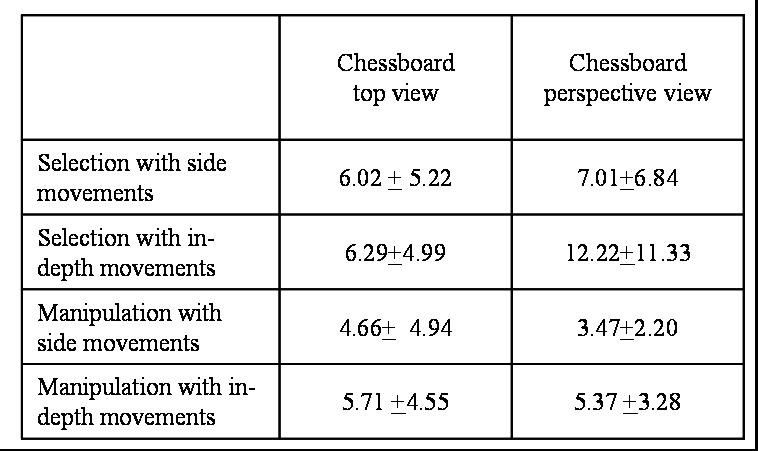
\includegraphics[width=.7\textwidth]{table.jpg}
\end{table}

\section{Images}

All images and illustrations should be in black-and-white, or gray tones,
excepting for the papers that will be electronically available (on CD-ROMs,
internet, etc.). The image resolution on paper should be about 600 dpi for
black-and-white images, and 150-300 dpi for grayscale images.  Do not include
images with excessive resolution, as they may take hours to print, without any
visible difference in the result. 

\section{References}

Bibliographic references must be unambiguous and uniform.  We recommend giving
the author names references in brackets, e.g. \cite{knuth:84},
\cite{boulic:91}, and \cite{smith:99}.

The references must be listed using 12 point font size, with 6 points of space
before each reference. The first line of each reference should not be
indented, while the subsequent should be indented by 0.5 cm.

\bibliographystyle{sbc}
\bibliography{sbc-template}

\end{document}
